\documentclass{beamer}
\usepackage{amsmath}
\usepackage[english]{babel} %set language; note: after changing this, you need to delete all auxiliary files to recompile
\usepackage[utf8]{inputenc} %define file encoding; latin1 is the other often used option
\usepackage{csquotes} % provides context sensitive quotation facilities
\usepackage{graphicx} %allows for inserting figures
\usepackage{booktabs} % for table formatting without vertical lines
\usepackage{textcomp} % allow for example using the Euro sign with \texteuro
\usepackage{stackengine}
\usepackage{wasysym}
\usepackage{tikzsymbols}
\usepackage{textcomp}
% ELIMINAR COMANDOS DE NAVEGACION%%%%%%%%%%%
\setbeamertemplate{navigation symbols}

%\newcommand{\bubblethis}[2]{
 %       \tikz[remember picture,baseline]{\node[anchor=base,inner sep=0,outer sep=0]%
 %       (#1) {\underline{#1}};\node[overlay,cloud callout,callout relative pointer={(0.2cm,-0.7cm)},%
 %       aspect=2.5,fill=yellow!90] at ($(#1.north)+(-0.5cm,1.6cm)$) {#2};}%
 %   }%
%\tikzset{face/.style={shape=circle,minimum size=4ex,shading=radial,outer sep=0pt,
 %       inner color=white!50!yellow,outer color= yellow!70!orange}}

%% Some commands to make the code easier
\newcommand{\emoticon}[1][]{%
  \node[face,#1] (emoticon) {};
  %% The eyes are fixed.
  \draw[fill=white] (-1ex,0ex) ..controls (-0.5ex,0.2ex)and(0.5ex,0.2ex)..
        (1ex,0.0ex) ..controls ( 1.5ex,1.5ex)and( 0.2ex,1.7ex)..
        (0ex,0.4ex) ..controls (-0.2ex,1.7ex)and(-1.5ex,1.5ex)..
        (-1ex,0ex)--cycle;}
\newcommand{\pupils}{
  %% standard pupils
  \fill[shift={(0.5ex,0.5ex)},rotate=80] 
       (0,0) ellipse (0.3ex and 0.15ex);
  \fill[shift={(-0.5ex,0.5ex)},rotate=100] 
       (0,0) ellipse (0.3ex and 0.15ex);}

\newcommand{\emoticonname}[1]{
  \node[below=1ex of emoticon,font=\footnotesize,
        minimum width=4cm]{#1};}
\usepackage{scalerel}
\usetikzlibrary{positioning}
\usepackage{xcolor,amssymb}
\newcommand\dangersignb[1][2ex]{%
  \scaleto{\stackengine{0.3pt}{\scalebox{1.1}[.9]{%
  \color{red}$\blacktriangle$}}{\tiny\bfseries !}{O}{c}{F}{F}{L}}{#1}%
}
\newcommand\dangersignw[1][2ex]{%
  \scaleto{\stackengine{0.3pt}{\scalebox{1.1}[.9]{%
  \color{red}$\blacktriangle$}}{\color{white}\tiny\bfseries !}{O}{c}{F}{F}{L}}{#1}%
}
\usepackage{fontawesome} % Social Icons
\usepackage{epstopdf} % allow embedding eps-figures
\usepackage{tikz} % allows drawing figures
\usepackage{amsmath,amssymb,amsthm} %advanced math facilities
\usepackage{lmodern} %uses font that support italic and bold at the same time

\usepackage{tikz}

\usepackage{tcolorbox}

\usefonttheme[onlymath]{serif} %set math font to serif ones

\definecolor{beamerblue}{rgb}{0.2,0.2,0.7} %define beamerblue color for later use

%%% defines highlight command to set text blue
\newcommand{\highlight}[1]{{\color{blue}{#1}}}


%%%%%%% commands defining backup slides so that frame numbering is correct

\newcommand{\backupbegin}{
   \newcounter{framenumberappendix}
   \setcounter{framenumberappendix}{\value{framenumber}}
}
\newcommand{\backupend}{
   \addtocounter{framenumberappendix}{-\value{framenumber}}
   \addtocounter{framenumber}{\value{framenumberappendix}}
}

%%%% end of defining backup slides

%Specify figure caption, see also http://tex.stackexchange.com/questions/155738/caption-package-not-working-with-beamer
\setbeamertemplate{caption}{\insertcaption} %redefines caption to remove label "Figure".
%\setbeamerfont{caption}{size=\scriptsize,shape=\itshape,series=\bfseries} %sets figure  caption bold and italic and makes it smaller


\usetheme{Boadilla}

\usepackage{hyperref}

% --------------------
% Overall information
% --------------------
\title[Economía I]{Economía I \vspace{4mm}
\\ Magistral 8: Teoría de Juegos}
\date{}
\author[Riottini]{Franco Riottini}
\vspace{0.4cm}
\institute[]{Universidad de San Andrés} 



\begin{document}

\begin{frame}
\titlepage
\centering

\includegraphics[scale=0.2]{../Figures/logoUDESA.jpg} 
\end{frame}

\begin{frame}
\frametitle{Dilemas Sociales}
\begin{itemize}
    \item Una parte de la economía estudia este tipo de dilemas sociales
    \item Para modelar estos dilemas sociales y distintos tipos de interacciones sociales se suele utilizar lo que se conoce como teoría de juegos
    \end{itemize}
\end{frame}

\begin{frame}{Teoría de juegos}
    \begin{itemize}
        \item Estudia de manera formal y abstracta las decisiones óptimas que deben tomar diversos adversarios en conflicto
        \item Es el estudio matemático de la toma de decisiones, del conflicto y la estrategia en situaciones sociales
        \item Jugadores que toman decisiones que se consideran estratégicas
        \begin{itemize}
            \item los jugadores son entes racionales (no necesariamente humanos)
            \item los entes que participan en el juego actúan teniendo en cuenta las acciones que tomarían los demás
        \end{itemize}
    \end{itemize}
\end{frame}


\begin{frame}{Estudiando juegos}
    \begin{itemize}
        \item El término ``juegos'' refiere básicamente a modelos de interacción estratégica
        \begin{itemize}
            \item Es decir, modelos donde las personas involucradas en una interacción social saben que sus acciones afectan a otros y viceversa
            \begin{itemize}
                \item En este contexto, una estrategia es una acción (o un curso de acción) que puede tomar una persona cuando es consciente de esta dependencia mutua de los resultados
            \end{itemize}
        \end{itemize}
        \item ¿Cómo analizamos interacciones sociales?
        \begin{itemize}
            \item Definimos las características de un juego
            \item Obtenemos ‘modos de jugar’
            \begin{itemize}
                \item que cumplen con ciertos criterios y nos ayudan a entender si esa manera de jugar es una buena
            \end{itemize}
        \end{itemize}
    \end{itemize}
\end{frame}

\begin{frame}
    \frametitle{Elementos de un juego}
    \begin{itemize}
        \item \textbf{Los jugadores:} quién está interactuando con quién.\vspace{4mm}
        \item \textbf{Las estrategias viables:} qué acciones están abiertas a los jugadores.\vspace{4mm}
        \item \textbf{La información:} lo que cada jugador sabe al tomar su decisión.\vspace{4mm}
        \item \textbf{Los beneficios:} cuáles serán los resultados para cada una de las posibles combinaciones de acciones.\vspace{4mm}
    \end{itemize}
\end{frame}

% \begin{frame}
%     \frametitle{Tipos de juegos}
%     \begin{itemize}
%         \item Juegos simultáneos: donde se toma una decisión one-shot.\vspace{4mm}
%         \item Juegos secuenciales: donde los jugadores toman sus decisiones de forma consecutiva.\vspace{4mm}
%     \end{itemize}
% \end{frame}


% \begin{frame}
%     \frametitle{ Estudiando juegos}
%     \begin{itemize}
%         \item “The Economy” presenta un problema de división de trabajo
%     \begin{itemize}
%         \item Dos individuos deben decidir qué producir, con el riesgo de terminar produciendo lo mismo
%             \begin{itemize}
%                 \item ¿Por qué es esto un problema?
%                 \item Por alguna razón, no se pueden poner de acuerdo
%                 \item Toman decisiones en forma independiente
%                 \item Juegan una sola vez   
%             \end{itemize}
%         \item ¿Arroz o mandioca?
%             \begin{itemize}
%                 \item Asumimos que ninguno puede producir ambos...
%                 \item ... y que Bala es mejor produciendo arroz, mientras que Anil es mejor produciendo mandioca
%             \end{itemize}
%     \end{itemize}
% \end{frame}

% \begin{frame}{El juego de Anil y Bala}
%     \begin{itemize}
%         \item Jugadores
%         \begin{itemize}
%             \item Anil y Bala, dos agricultores que deciden en qué cultivo especializarse
%         \end{itemize}
%         \item Estrategias viables
%         \begin{itemize}
%             \item Arroz o mandioca
%         \end{itemize}
%         \item Información
%         \begin{itemize}
%             \item Ningún agricultor sabe lo que el otro elige
%         \end{itemize}
%         \item Pagos
%         \begin{itemize}
%             \item Dependerá de los precios de mercado y de la calidad de la tierra
%         \end{itemize}
%     \end{itemize}
% \end{frame}

% \begin{frame}{Escenarios}
%     \centering
%     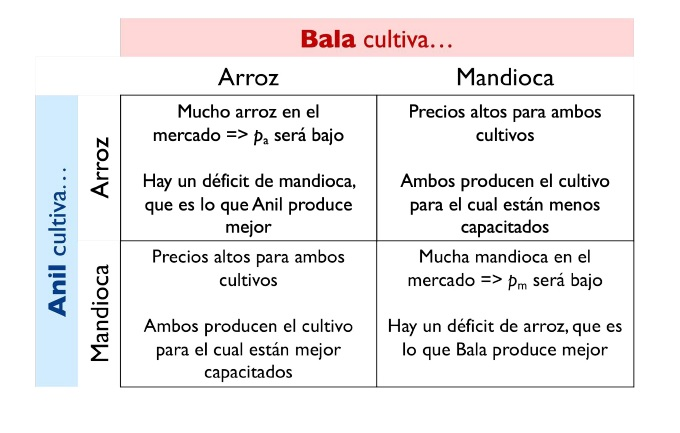
\includegraphics[scale=0.65]{../Figures/Tema_03_7_bala.jpg}
% \end{frame}

% \begin{frame}{Construyendo la matriz de pagos}
%     \centering
%     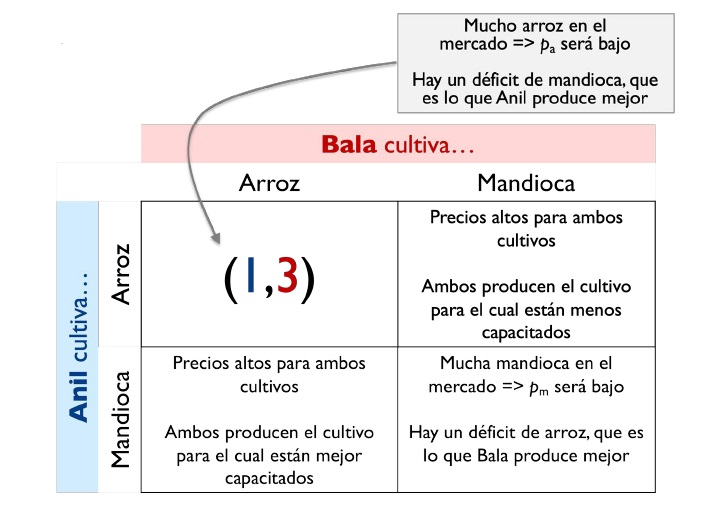
\includegraphics[scale=0.6]{../Figures/Tema_03_8_bala.jpg}
% \end{frame}

% \begin{frame}
%     \frametitle{Construyendo la matriz de pagos}
%     \centering
%     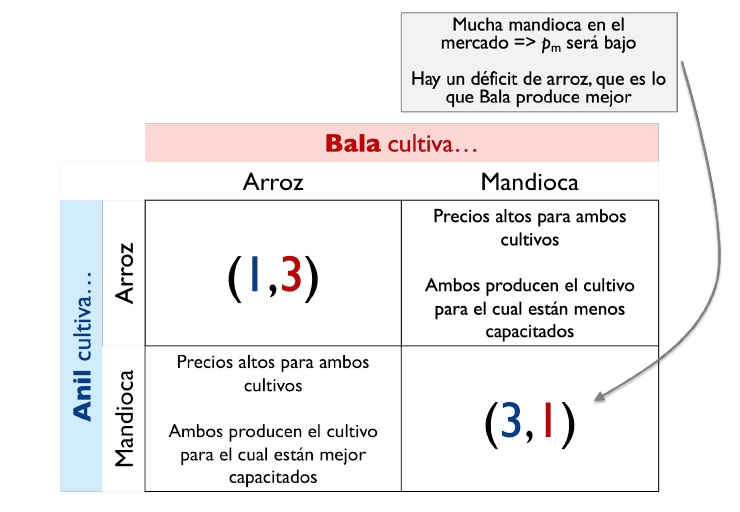
\includegraphics[scale=0.6]{../Figures/Tema_03_9_bala.jpg}
% \end{frame}

% \begin{frame}
%     \frametitle{ Construyendo la matriz de pagos}
%     \centering
%     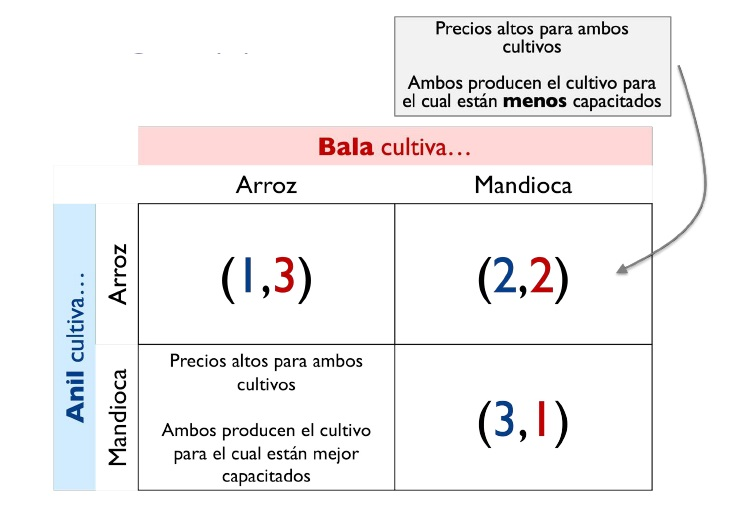
\includegraphics[scale=0.6]{../Figures/Tema_03_10_bala.jpg}
% \end{frame}

% \begin{frame}
%     \frametitle{Construyendo la matriz de pagos}
%     \centering
%     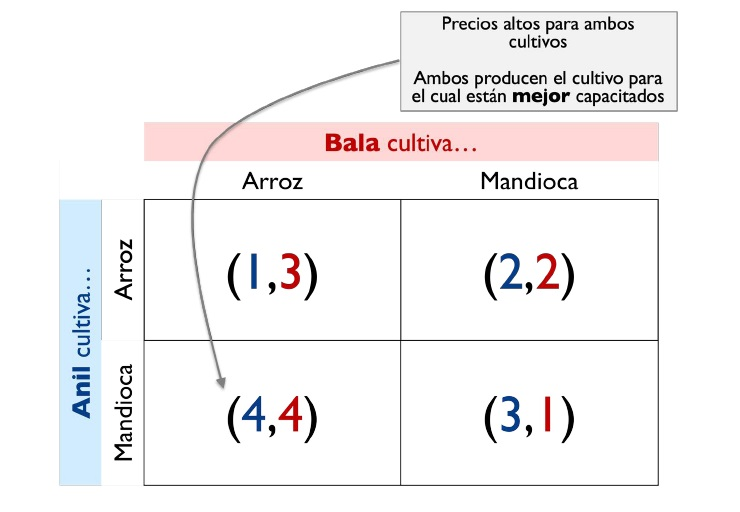
\includegraphics[scale=0.6]{../Figures/Tema_03_11_bala.jpg}
% \end{frame}

% \begin{frame}
%     \frametitle{Matriz de pagos}
%     \centering
%     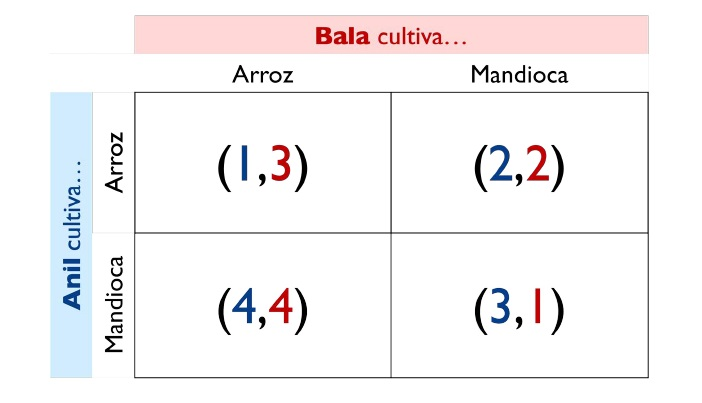
\includegraphics[scale=0.6]{../Figures/Tema_03_12_bala.jpg}
% \end{frame}

% \begin{frame}
%     \frametitle{¿Cómo pensamos el problema?}
%     \begin{itemize}
%         \item ¿Cuál es la mejor respuesta de cada individuo?
%         \begin{itemize}
%             \item Aquella estrategia que brinda los mayores pagos, dada la estrategia seleccionada por la otra persona
%         \end{itemize}
%         \item A veces, existe una estrategia dominante
%         \begin{itemize}
%             \item Esta es una mejor respuesta a todas las posibles estrategias de otro jugador
%         \end{itemize}
%         \item Si se encuentra un resultado donde cada individuo juega su estrategia dominante, entonces nos encontramos con un equilibrio en estrategia dominante
%     \end{itemize}
% \end{frame}

% \begin{frame}
%     \frametitle{ ¿Cómo piensa Anil?}
%     \centering
%     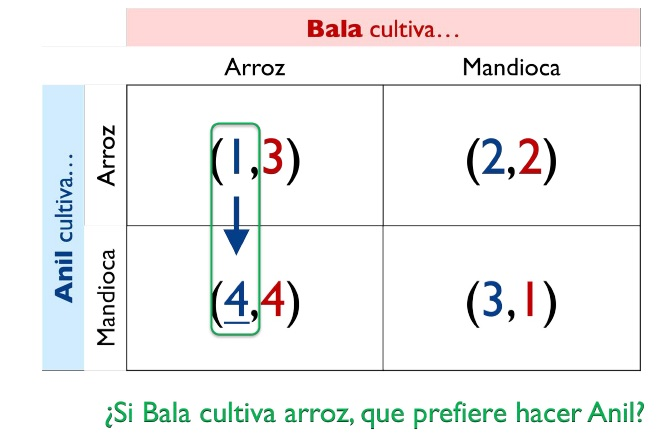
\includegraphics[scale=0.6]{../Figures/Tema_03_13_bala.jpg}
% \end{frame}

% \begin{frame}
%     \frametitle{ ¿Cómo piensa Anil?}
%     \centering
%     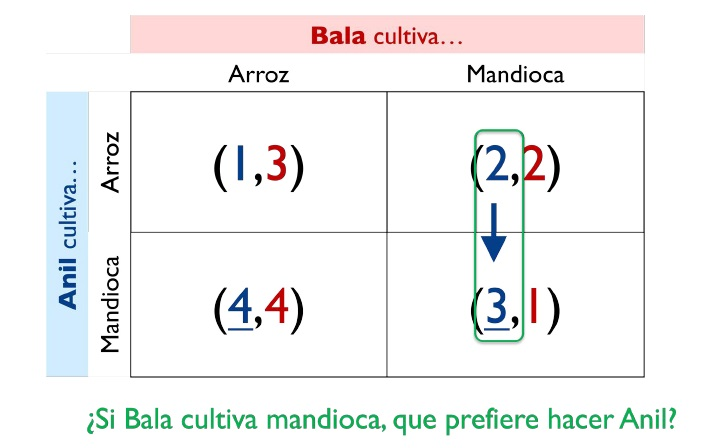
\includegraphics[scale=0.6]{../Figures/Tema_03_14_bala.jpg}
% \end{frame}

% \begin{frame}
%     \frametitle{ ¿Qué hace Anil?}
%     \centering
%     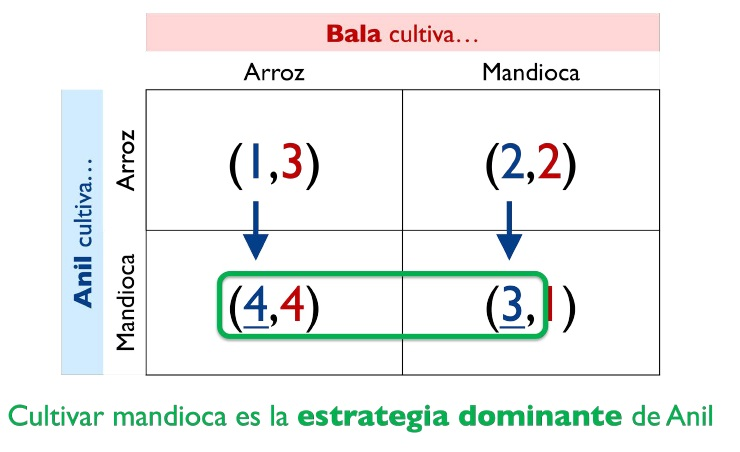
\includegraphics[scale=0.6]{../Figures/Tema_03_15_bala.jpg}
% \end{frame}

% \begin{frame}
% \frametitle{ ¿Cómo piensa Bala?}
% \centering
% 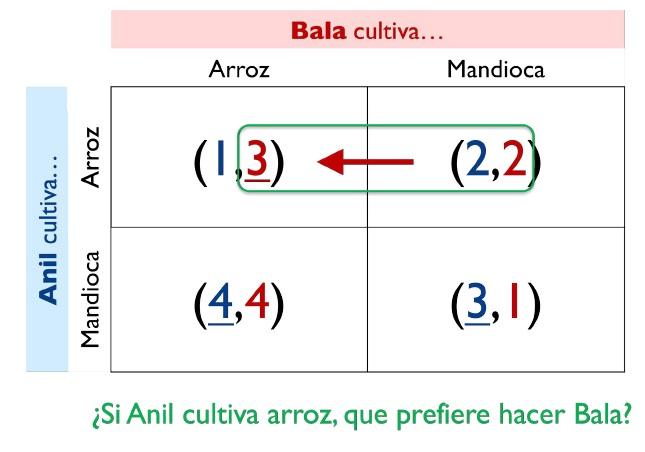
\includegraphics[scale=0.6]{../Figures/Tema_03_16_bala.jpg}
% \end{frame}

% \begin{frame}
% \frametitle{ ¿Cómo piensa Bala?}
% \centering
% 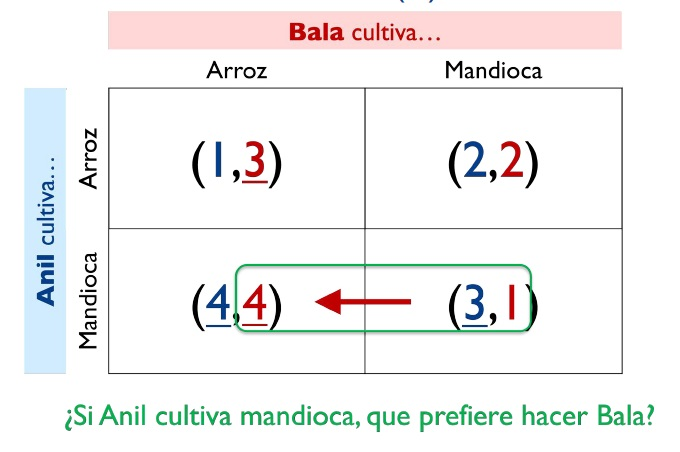
\includegraphics[scale=0.6]{../Figures/Tema_03_17_bala.jpg}
% \end{frame}

% \begin{frame}
% \frametitle{ ¿Qué hace Bala?}
% \centering
% 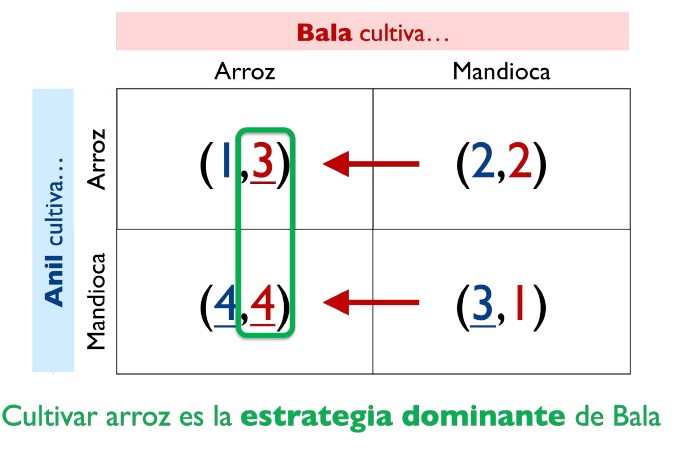
\includegraphics[scale=0.6]{../Figures/Tema_03_18_bala.jpg}
% \end{frame}

% \begin{frame}
% \frametitle{Equilibrio}
% \centering
% 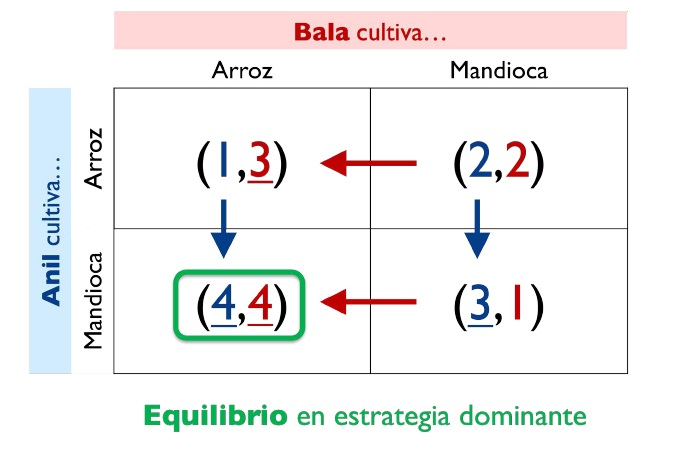
\includegraphics[scale=0.6]{../Figures/Tema_03_19_bala.jpg}
% \end{frame}

% \begin{frame}
%     \frametitle{Teoría de juegos y estrategia competitiva}
%     \begin{block}{Equilibrio de Nash}
%     Un equilibrio de Nash es un par de estrategias, una para cada jugador, en las que cada estrategia es la mejor respuesta dado lo que hace el otro
%     \end{block}
%     \vspace{5mm}
%     En equilibrio, cada jugador está haciendo lo mejor que puede, dado lo que el otro jugador también lo está haciendo
% \end{frame}


% \begin{frame}
%     \frametitle{Otro juego: Dilema del prisionero}
%     \begin{itemize}
%         \item Dos sospechosos son arrestados y acusados de un delito
%         \item La policía no tiene evidencia suficiente para condenar a los sospechosos a menos que uno confiese
%         \item La policía encierra a los sospechosos en celdas separadas y les explica las consecuencias derivadas de las decisiones que formen
%     \end{itemize}
% \end{frame}

% \begin{frame}
%     \frametitle{Dilema de los prisioneros}
%     \begin{itemize}
%         \item Si ninguno confiesa, ambos serán condenados por un delito menor sentenciados a un mes de cárcel
%         \item Si ambos, confiesan serán sentenciados a seis meses de cárcel
%         \item Finalmente, si uno confiesa y el otro no, el que confiesa será puesto en libertad inmediatamente y el otro será sentenciado a nueve meses en prisión, seis por el delito y tres más por obstrucción a la justicia
%     \end{itemize}
% \end{frame}

% \begin{frame}
% \frametitle{Dilema de los prisioneros}
% \begin{table}
%      \begin{tabular}{cc|c|c|}
%       & \multicolumn{1}{c}{} & \multicolumn{2}{c}{Preso $2$}\\
%       & \multicolumn{1}{c}{} & \multicolumn{1}{c}{No confesar}  & \multicolumn{1}{c}{Confesar} \\\cline{3-4}
%       \multirow{}{Preso $1$}  & No Confesar & $(-1,-1)$ & $(-9,0)$ \\\cline{3-4}
%       & Confesar & $(0,-9)$ & $(-6,-6)$ \\\cline{3-4}
%     \end{tabular}
%   \end{table}
% \end{frame}

%\begin{frame}
%\frametitle{Dilema de los prisioneros}
%\begin{itemize}
%\item Cada jugador cuenta con dos estrategias posibles: confesar y no confesar. 
%\item Las ganancias de los dos jugadores cuando eligen un par concreto de estrategias aparecen en la casilla correspondiente de la matriz binaria. 
%\item Por convención, la ganancia del llamado jugador-fila (Preso 1) es la primera ganancia, seguida, por la ganancia del jugador columna (Preso 2). 
%\end{itemize}
%\end{frame}


%\begin{frame}
%\frametitle{ Otro juego}
%\begin{itemize}
%    \item Dos empresas productoras de \textit{smartphones}
%    \item Comparten por igual el mercado de un país por, digamos, \$8 millones
%    \item Enfrentan el problema de invertir en publicidad
%        \begin{itemize}
%        \item Si ambos invierten en publicidad, mantienen su proporción del mercado inalterada
%        \item Si uno de ellos invierte  \$1 millón, se queda con $\frac{3}{4}$ del mercado
%        \end{itemize}
%    \item ¿Cómo analizamos este caso?    
%\end{itemize}
%\end{frame}

%\begin{frame}
%\frametitle{ El juego de Apple y Samsung}
%\begin{itemize}
%    \item Jugadores
%        \begin{itemize}
%        \item Apple y Samsung, dos compañías que quieren maximizar su participación en el mercado
%        \end{itemize}
%    \item Estrategias viables
%        \begin{itemize}
%        \item Publicitar o no publicitar
%        \end{itemize}
%    \item Información
%        \begin{itemize}
%        \item Ambos tienen la misma información, y ninguno puede ver la decisión del otro antes de jugar
%        \end{itemize}
%    \item Pagos
%        \begin{itemize}
%        \item Dependerá del costo de publicidad y el mercado
%        \end{itemize}
%\end{itemize}
%\end{frame}

%\begin{frame}
%\frametitle{ Matriz de pagos}
%\centering
%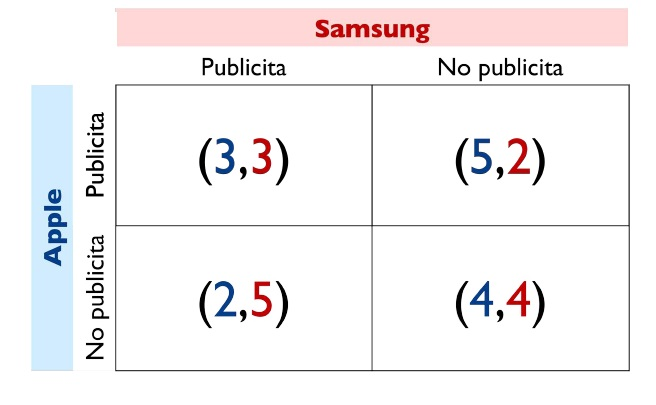
\includegraphics[scale=0.6]{../Figures/Tema_03_20_bala.jpg}
%\end{frame}

%\begin{frame}
%\frametitle{ Equilibrio}
%\centering
%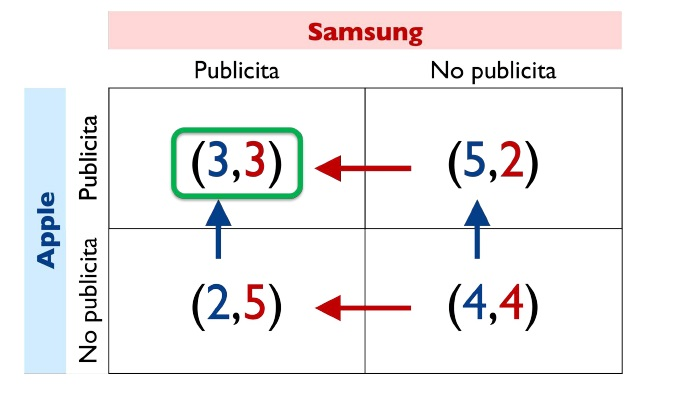
\includegraphics[scale=0.6]{../Figures/Tema_03_21_bala.jpg}
%\end{frame}

% \begin{frame}
% \frametitle{Dilema del prisionero}
%     \begin{itemize}
%         \item Típicamente, un juego con un equilibrio en estrategia dominante donde el resultado son pagos individuales y totales inferiores a otras estrategias posibles
%     \end{itemize}
%     \textbf{El resultado socialmente óptimo no es alcanzado} \vspace{2mm}
%     \begin{itemize}
%         \item Este tipo de dilema es útil para representar una serie de problemáticas sociales
%         \begin{itemize}
%         \item Desde temas ambientales hasta conflictos en la provisión de algunos tipos de bienes
%         \end{itemize}
%     \end{itemize}
% \end{frame}

% \begin{frame}
% \frametitle{Problemas y soluciones}
% \begin{itemize}
%     \item ¿Por qué se llega a este tipo de resultado y en qué forma se puede amenorar o solucionar?
%     \item Algunas razones (y soluciones)
%         \begin{itemize}
%         \item Los jugadores sólo se preocupan por sus propios beneficios \\
%         - Podemos introducir preferencias sociales
%         \item Nadie puede hacer que los jugadores paguen por las consecuencias de sus acciones sobre los demás \\
%         - Juegos repetidos, normas sociales y castigo de pares
%         \item Los jugadores no pueden coordinar sus acciones con antelación \\
%         - Cambiar las reglas del juego (instituciones y políticas)
%         \end{itemize}
% \end{itemize}
% \end{frame}

% \begin{frame}
% \frametitle{Asfaltando la calle}
% \begin{itemize}
%     \item Dos familias viven en una calle de tierra (Álvarez y Benítez)
%     \item Ambas se beneficiarían si se asfaltara la calle
%         \begin{itemize}
%         \item Por ejemplo, tendrían que gastar menos en arreglo y limpieza de sus autos por \$15.000
%         \end{itemize}
%     \item Enfrentan el problema de invertir en el asfalto
%         \begin{itemize}
%         \item El costo de asfaltar la calle es de \$20.000
%         \item Puede pagarlo una u otra familia, o las dos juntas
%         \end{itemize}
% \item ¿Cómo analizamos este caso?
% \end{itemize}
% \end{frame}

% \begin{frame}
% \frametitle{El juego del asfalto}
% \begin{itemize}
%     \item Jugadores
%         \begin{itemize}
%         \item Familias Álvarez y Benítez
%         \end{itemize}
%     \item Estrategias viables
%         \begin{itemize}
%         \item Pagar o no pagar por el asfalto
%         \end{itemize}
%     \item Información
%         \begin{itemize}
%         \item Ambos tienen la misma información, y ninguno puede ver la decisión del otro antes de jugar
%         \end{itemize}
%     \item Pagos
%         \begin{itemize}
%         \item Dependerá del ahorro en arreglos del auto y la contribución al costo del asfalto
%         \end{itemize}
% \end{itemize}
% \end{frame}

% \begin{frame}
% \frametitle{ Pagando por el asfalto}
% \centering
% 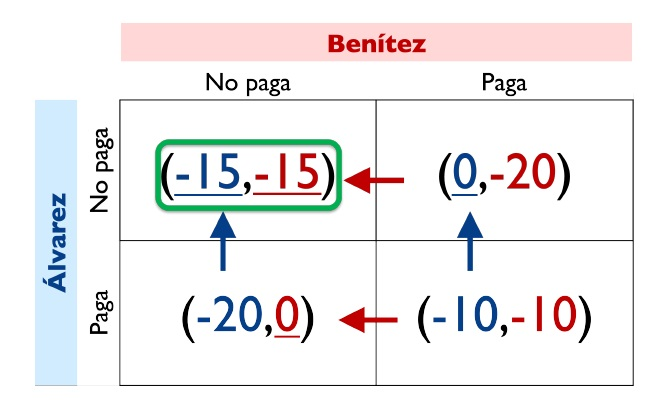
\includegraphics[scale=0.6]{../Figures/Tema_03_27_abel.jpg}
% \end{frame}

% \begin{frame}
% \frametitle{El problema del bien público}
% \begin{itemize}
%     \item Existe un tipo de bien, usualmente llamado bien público, con dos características distintivas:
%     \begin{itemize}
%         \item Es no rival \\
%         - Su uso por una persona no perjudica o impide el uso simultáneo por parte de otros individuos
%         \item Es no excluyente \\
%         - No se puede impedir ser utilizado
%     \end{itemize}
%     \item El dilema del prisionero ilustra un problema de los bienes públicos: pueden no producirse
%     \begin{itemize}
%         \item Dadas sus característica, existe la posibilidad de hacer free-riding \\
%         - ¡No contribuir es la estrategia dominante!
%     \end{itemize}
% \end{itemize}
% \end{frame}

% \begin{frame}
% \frametitle{ Pagando por los costos que uno genera}
% \begin{itemize}
%     \item Tanto en el caso del asfalto, como en el de los pesticidas elaborado en “The Economy”: \\
% \end{itemize}
% \vspace{5mm}
% \textbf{Es difícil hacer pagar a los jugadores por la
% consecuencias de sus acciones sobre los demás}
% \end{frame}

% \begin{frame}
% \frametitle{ Mitigando el problema}
% \begin{itemize}
%     \item Mecanismos ayudan a reducir el problema
%     \begin{itemize}
%         \item Juegos repetidos \\
%         - Repetición contribuye a la cooperación: las consecuencias en el futuro hacen la estrategia egoísta sub-óptima
%         \item Normas sociales \\
%         - Reglas que indican como actuar en contextos particulares \\
%         - Individuos a veces incurren en considerables costos para castigar a pares que violan normas sociales o llevan a cabo acciones que consideran injustas (¿gusto por equidad?)
%     \end{itemize}
% \end{itemize}
% \end{frame}

% \begin{frame}
% \frametitle{ Aprendiendo sobre preferencias}
% \begin{itemize}
%     \item Los economistas utilizan a veces experimentos para aprender sobre las preferencias
%     \begin{itemize}
%         \item En el laboratorio: \\
%         - Se puede controlar las decisiones de los participantes y sus resultados \\
%         - Se puede crear un grupo de control / tratamiento para la comparación \\
%         - Los resultados pueden ser replicados \\
%         - Se pueden controlar otras variables
%         \item En el campo \\
%         - Algunos experimentos de laboratorio no pueden predecir la toma de decisiones en el mundo real \\
%         - El campo provee un contexto más realista en el que las personas toman decisiones
%     \end{itemize}
% \end{itemize}
% \end{frame}

% \begin{frame}
% \frametitle{ El dilema de la guardería}
% \begin{itemize}
%     \item Un experimento `real' (`field experiment')
%        \begin{itemize}
%        \item Se introdujo una multa a la llegada tarde de los padres... con un resultado no esperado \\
%         - ¡Más padres empezaron a llegar tarde!
%         \end{itemize}
%     \item ¿Por qué?
%         \begin{itemize}
%         \item Antes del experimento, llegar tarde era `incorrecto' 
%         \item El tiempo de los maestros pasó a tener un valor definido \\
%         - El precio del retardo, que los padres podían estar dispuestos a pagar o no \\ 
%         \item En este caso, se dice que los incentivos hicieron un crowding out de las preferencias sociales
%     \end{itemize}
% \end{itemize}
% \end{frame}

% \begin{frame}
% \frametitle{ En el campo ... con padres y niños}
% \centering
% 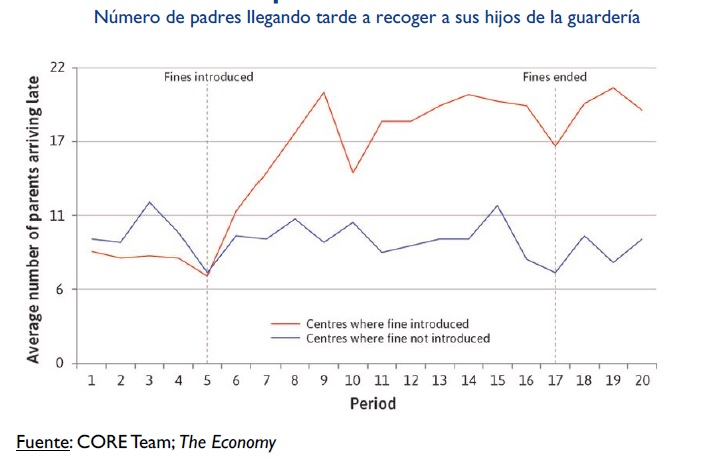
\includegraphics[scale=0.6]{../Figures/Tema_03_28_guarderia.jpg}
% \end{frame}

% \begin{frame}
% \frametitle{Negociando}
% \begin{itemize}
%     \item La cooperación es posible aun cuando agentes 
%     actúan en forma independiente
%     \begin{itemize}
%         \item En muchos de los ejemplos que discutimos no fue necesario que los individuos se pusieran de acuerdo \\
%         - A veces las condiciones del juego ayudaban (con Anil y Bala), o si se repetía el juego, o si permitía sancionar a los que no colaboraban
%     \end{itemize}
%     \item Pero la negociación es otra herramienta para conseguir un acuerdo mutuamente beneficioso
%     \begin{itemize}
%         \item Más fácil decirlo que hacerlo \\
%         - ¿Cómo repartir los costos y beneficios de la interacción?
%     \end{itemize}
% \end{itemize}
% \end{frame}

% \begin{frame}
% \frametitle{Motivando preferencias sociales}
% \begin{itemize}
%         \item Altruismo
%         \begin{itemize}
%             \item Una persona puede ser altruista y preocuparse de la felicidad (o sobre algún otro aspecto del bienestar) de los demás
%         \end{itemize}
%         \item Equidad
%         \begin{itemize}
%             \item La importancia de distribuir recursos en forma justa \\
%             - Motivación por lo que los economistas llaman `aversión por la desigualdad'
%         \end{itemize}
%         \item Reciprocidad
%         \begin{itemize}
%             \item Existencia de preferencias recíprocas \\
%             - Si en el pasado han sido generosos con nosotros, merecemos tratar en forma generosa
%         \end{itemize}
% \end{itemize}
% \end{frame}

% \begin{frame}
% \frametitle{ Juego del ultimátum}
% \begin{itemize}
%         \item Una herramienta muy utilizada para estudiar preferencias sociales es el juego del ultimátum
%         \begin{itemize}
%             \item ü Dos jugadores, seleccionados aleatoriamente \\ 
%             - Proponente \\
%             - Receptor
%             \item El proponente recibe algo de valor (típicamente dinero) y debe ofrecerle al receptor una parte \\
%             - Que puede ser cualquier cosa entre todo y nada \\
%             - El receptor sabe cuán grande es el total
%             \item Una vez que el receptor escucha la oferta, decide si la acepta o no \\
%             - Si la oferta es rechazada, nadie recibe nada \\
%             - Si es aceptada, se reparte como sugirió el proponente
%         \end{itemize}
% \end{itemize}
% \end{frame}

% \begin{frame}
% \frametitle{ Juego secuencial}
% \centering
% 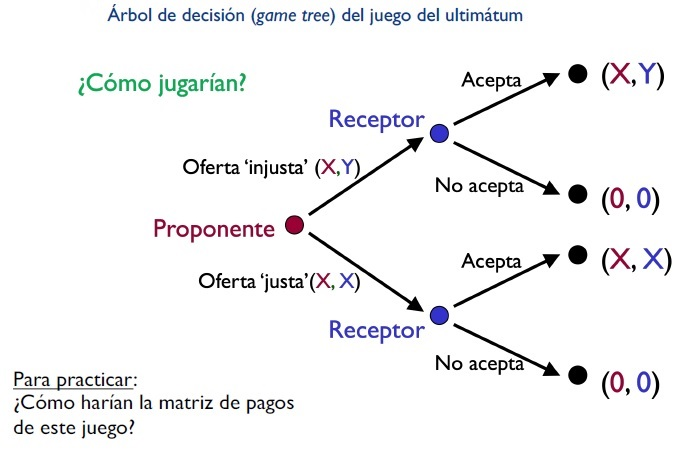
\includegraphics[scale=0.6]{../Figures/Tema_03_29_arbol.jpg}
% \end{frame}

% \begin{frame}
% \frametitle{ Agricultores versus estudiantes}
% \centering
% 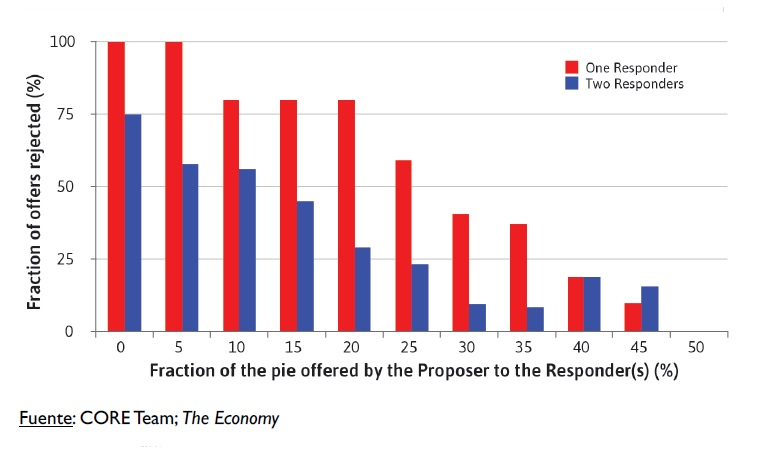
\includegraphics[scale=0.6]{../Figures/Tema_03_32_ultimatum.jpg}
% \end{frame}

% \begin{frame}
% \frametitle{ ¿Cuál es el beneficio esperado?}
% \centering
% 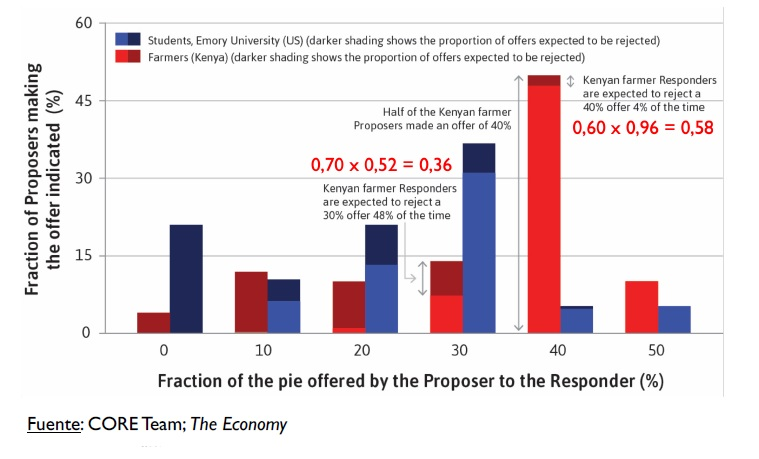
\includegraphics[scale=0.6]{../Figures/Tema_03_31_ultimatum.jpg}
% \end{frame}

% \begin{frame}
% \frametitle{ La batalla de los sexos}
% \begin{itemize}
%         \item Una pareja arregló para ir al cine
%         \begin{itemize}
%             \item Alberto y Beatriz
%         \end{itemize}
%         \item No recuerdan qué película iban a ver
%         \begin{itemize}
%             \item Alberto quería ir a ver una comedia romántica
%             \item Beatriz una de acción
%         \end{itemize}
%         \item Ambos prefieren ir al mismo lugar que desencontrarse
%         \item No tienen forma de comunicarse
%         \item ¿Cómo analizamos este caso?
% \end{itemize}
% \end{frame}

% \begin{frame}
% \frametitle{¿Y si hay competencia?}
% \centering
% 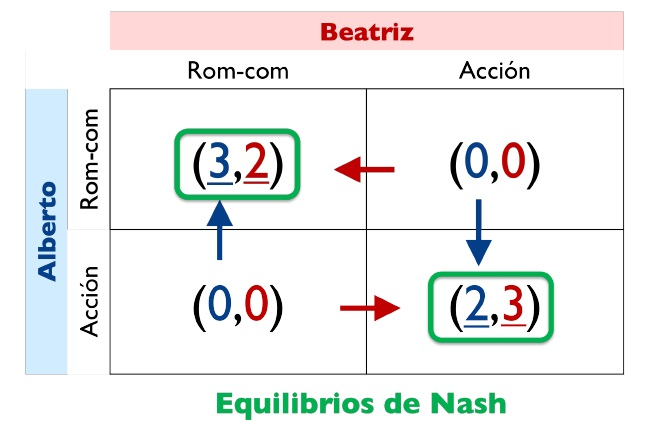
\includegraphics[scale=0.6]{../Figures/Tema_03_33_batallasexo.jpg}
% \end{frame}

% \begin{frame}
% \frametitle{Juegos de coordinación}
% \begin{itemize}
%         \item La batalla de los sexos es un típico juego de coordinación
%         \begin{itemize}
%             \item Ilustra situaciones que encontramos por doquier en la sociedad \\
%             - ¿Qué plataforma de social media usar? ¿De qué lado del camino conducir?
%         \end{itemize}
%         \item En este caso, el pago era idéntico en ambos equilibrios, pero puede que los jugadores queden atrapados en un mal equilibrio
%         \begin{itemize}
%             \item ¿Cómo se decide, por ejemplo, pasar de una tecnología a otra cuando la nueva implica un costo para el capitalista y para el trabajador?
%         \end{itemize}
% \end{itemize}
% \end{frame}

\end{document}